\documentclass[
 a4paper,twocolumn,showpacs,aip,groupedaddress,%
  eqsecnum,notitlepage,showkeys,cha,longbibliography,10pt
]{revtex4-1}
\usepackage[english]{babel}
\usepackage[utf8x]{inputenc}
\usepackage[T1]{fontenc}
\usepackage{amssymb}
\usepackage{amsmath,latexsym}
\usepackage{subcaption}
\usepackage{graphicx}
\usepackage{dcolumn}
\usepackage{tikz}
\usepackage{natbib}
\usepackage{float}
\usepackage[export]{adjustbox}
\usepackage{hyperref}
\usepackage{mathtools}
\usepackage{soul}
\DeclarePairedDelimiter\bra{\langle}{\rvert}
\DeclarePairedDelimiter\ket{\lvert}{\rangle}
\DeclarePairedDelimiterX\braket[2]{\langle}{\rangle}{#1 \delimsize\vert #2}

\newcommand*{\citen}[1]{%
  \begingroup
    \romannumeral-`\x % remove space at the beginning of \setcitestyle
    \setcitestyle{numbers}%
    \cite{#1}%
  \endgroup   
}

\usepackage[a4paper,top=1.8cm,bottom=1.8cm,left=1.5cm,right=1.5cm]{geometry}
\usepackage[skip=5pt, font=scriptsize, labelfont=bf, justification=raggedright]{caption}

\usepackage{titlesec}

\titlespacing\section{0pt}{12pt plus 4pt minus 2pt}{0pt plus 2pt minus 2pt}

\graphicspath{ {Images/} }

\begin{document}

\title{\LARGE{Prospects and Applications for Chip-Scale Atomic Clocks}}

\author{Lindsey Keary}
\affiliation{ 
Student Number : 17099595, l.keary.17@ucl.ac.uk, University College London
}
\date{\today}


\begin{abstract}

\end{abstract}


\maketitle

% \input{leadpara}

\input{intro}
\section{\label{sec:level1}Introduction}
Highly accurate and stable timing is vital for everyday applications such as navigation, communication and power distribution $^[$\citep{Knappe2007MEMSClocks}$^,$\citep{Mileti2017IntroductionClocks}$^]$. Since the redefinition of the SI second in 1967 using the ground sate caesium (Cs) atomic transition as the frequency reference, a variety of Cs beam atomic clocks were used as the time and frequency standard. However, as atomic trapping and laser cooling techniques became available atomic clock accuracy continued to improve rapidly. In 1998 laser-cooled fountain atomic clocks became the primary frequency standard with the current best accuracy of $\approx10^{-16}$   $^[$\citep{LombardiM.A.andHeavnerT.PandJefferts2007NISTSI}$^,$\citep{Guena2012ProgressLNE-SYRTE}$^]$. The primary standard has small applied adjustments to allow coordinated universal time (UTC) and international timekeeping $^[$\citep{Lombardi2002NISTServices}$^]$. Recently optical lattice and single ion optical clocks exceed fountain clocks performance, with accuracy of $\approx10^{-17}$. Optical clocks are being considered for the SI second redefinition, measurement of the earth's gravitational potential and the possibility of replacing the atomic clocks used in current global navigational satellite systems (GNSSs) as the efforts are made to make these clocks more transportable $^[$\citep{Gill2011WhenSecond}$^,$\citep{Margolis2014TimekeepersFuture}$^,$\citep{Margolis2010OpticalClocks}$^,$\citep{Godun2017TransportableTimes}$^]$.

%Despite the success of continued efforts to improve the performance of atomic clocks it comes at the penalty of size and power consumption. 

Primary standard and optical clocks far exceed the required stability and accuracy for military and commercial applications but they are not portable. Current commercially available chip-scale atomic clocks (CSACs) provide replacement of temperature compensated crystal oscillators (TCXO) for military applications and GNSS receivers with a 88 $\%$ short-term stability improvement $^[$\citep{Fernandez2017CSACPerformance.}$^]$. The availability of the commercial device is the outcome of the CSAC program launched by the Defense Advanced Research Projects Agency (DARPA) in 2001. This program focused on providing lightweight battery-operated atomic clocks for secure communication provided by time-ordered encryption key synchronisation and P(Y)-Code signal acquisition in the presence of local jamming of targeted GNSS receivers $^[$\citep{Lutwak2002TheInterrogation}$^,$\citep{Fruehauf2001FastClock.}$^]$. The aim of the program was to produce an atomic clock with a volume of 1 cm$^3$, stability of 10$^{-11}$ at one hour of integration time and power consumption below 30 mW $^[$\citep{LutwakR.DengJ.RileyW.andVargheseM.2004ThePackage}$^]$. DARPA has since launched the atomic clock with enhanced stability (ACES) program which aims to produce CSAC which meet the previous program requirements clocks but with an extended time stability $^[$\citep{DARPA2016Broad}$^]$. Potential commercial applications of CSACs include underwater sensing, financial trading time-keeping, enhanced GNSS receivers and improved synchronisation for digital communication and power distribution $^[$\citep{Lutwak2011PrinciplesClocks}$^,$\citep{KnappeChip-ScaleClock}$^]$. 



   


 





 














\section{\label{sec:level1}Theoretical Background}
The most stable frequency reference is atomic oscillators due to the unperturbed clock transition being indistinguishable between atoms. Atomic clocks most commonly employ alkali atoms due to their well studied single valence electronic structure, high vapor pressure at room temperature and the D-lines$^[$\citep{Steck1998CesiumData}$^]$ being accessible using diode lasers. 
\begin{figure}[t]
\centering
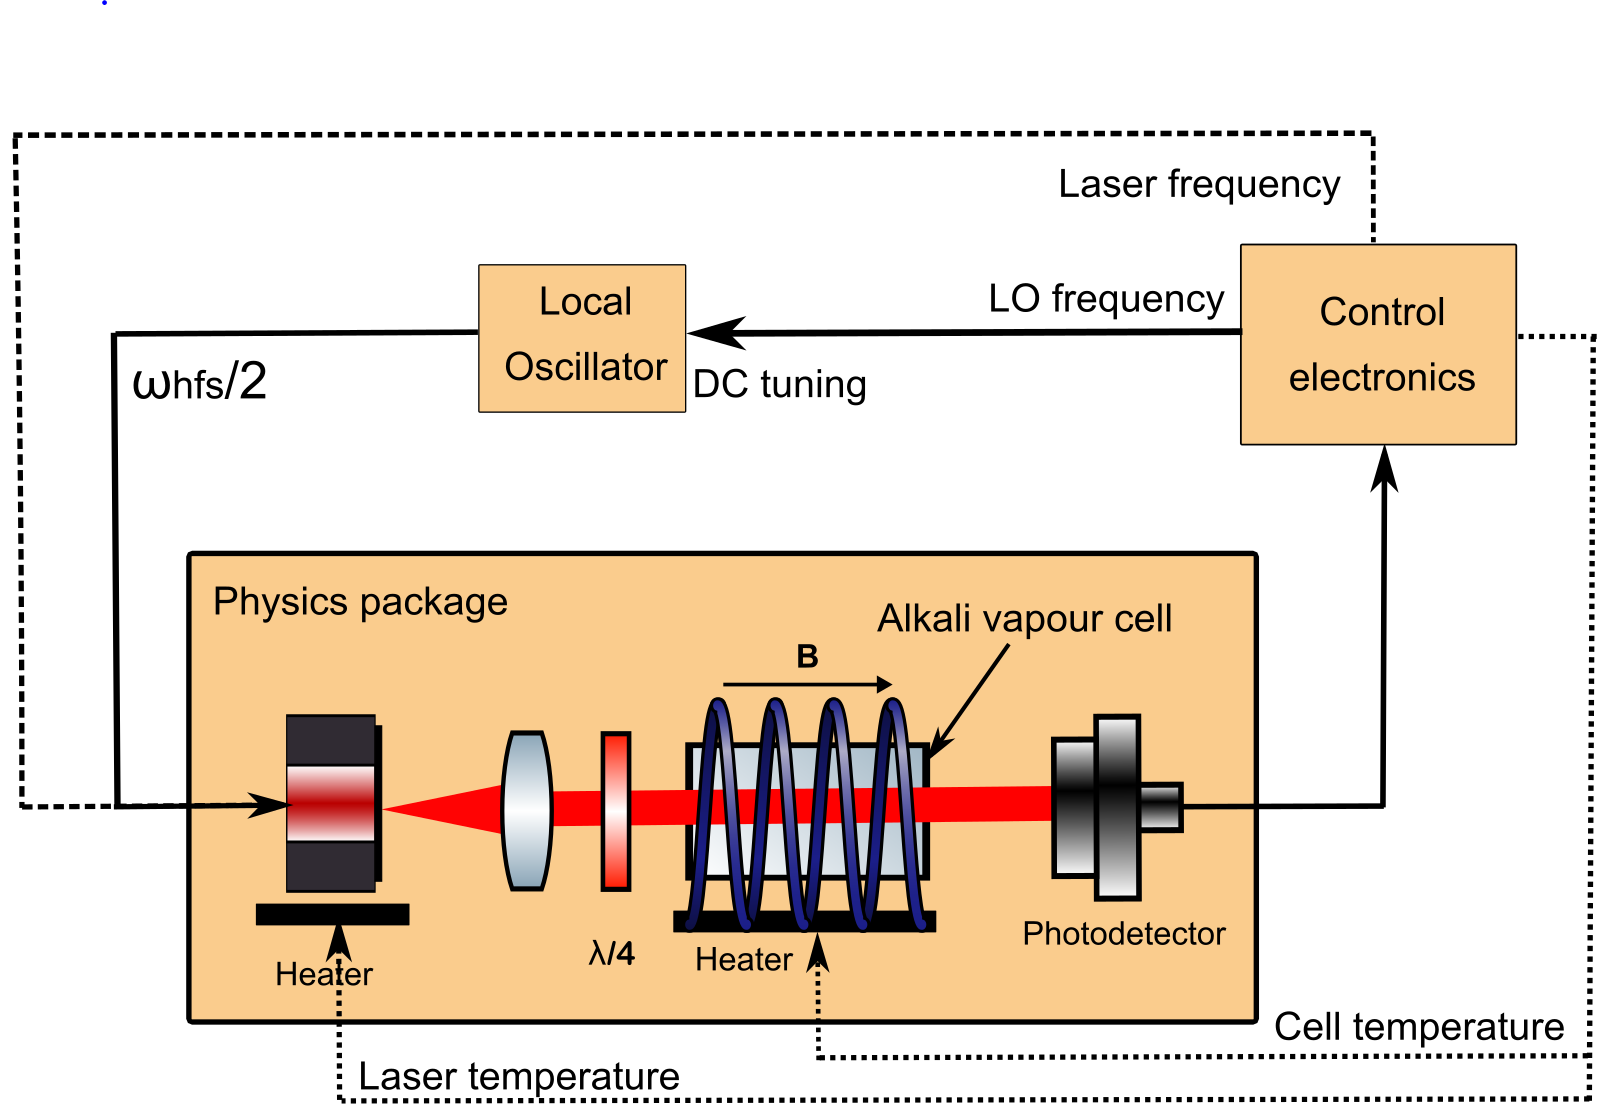
\includegraphics[width=0.45\textwidth,keepaspectratio]{expsetup}
\caption{\label{fig:expsetup}CSAC CPT schematic with the LO, physics package and control electronics.}
\end{figure}
The hyperfine states of the atoms are further split by the Zeeman effect into the Zeeman sub-levels, $m_{f}$ in the presence of a magnetic field. The clock states are chosen as the hyperfine ground states, F=3 and F=4 when $m_{f}$=0, ($\ket{F=3,m_{f}=0}$-$\ket{F=4,m_{f}=0}$). This is due to the transition between $m_{f}$=0 sub-levels being insensitive to magnetic fields to the first order. The transition frequency is calculated as the difference in energy between the clock states divided by Planck's constant $^[$\citep{Knappe2007MEMSClocks}$^,$\citep{LombardiM.A.andHeavnerT.PandJefferts2007NISTSI}$^,$\citep{Sherlock2009HowSpectroscopy}$^]$.

%cesium over rubidium for the alkali metal in the physics
%package permits the resonance cell to operate optimally at
%70-80°C and leads naturally to integrating the VCSEL with
%the resonance cell. firmware algorithms  


The local oscillator (LO), the physics package and the control electronics are the main components of a CSAC $^[$\citep{Knappe2007MEMSClocks}$^]$. The physics package contains the spectroscopic setup, for the case shown in Fig. (\ref{fig:expsetup}) the technique used is coherent population trapping (CPT). CPT transmission peak occurs at the frequency of the transition between the clock states and is used as the reference frequency for the LO. A small internal magnetic field $B$ is applied to the atoms in the vapor cell to deflect the $m_{f}\neq$0 sub-levels from the clock states. Magnetic shielding prevents external magnetic fields reaching the vapour cell. Miniaturisation of the physical package and the vapor cell is completed using the micro-electro-mechanical system (MEMS) technology $^[$\citep{Wang2014ReviewTrapping}$^]$. Buffer gas is added to the cell containing the alkali droplet to decrease the broadening due to collisions with the cell walls. However, pressure broadening shifts the hyperfine ground state but this can be corrected by adding a second buffer gas which produces an opposite pressure broadening ground state shift $^[$\citep{Lutwak2002TheInterrogation}$^]$. The vertical-cavity surface-emitting laser (VCSEL) is used due to the high modulation bandwidth $^[$\citep{Knappe2007MEMSClocks}$^]$. The control electronics are used to apply corrections to the laser frequency, LO frequency, laser temperature and vapour cell temperature. The laser frequency and the cell temperature are controlled using servo loops. 


\subsection{Coherent population trapping (CPT)}


\begin{figure}[t]
\centering
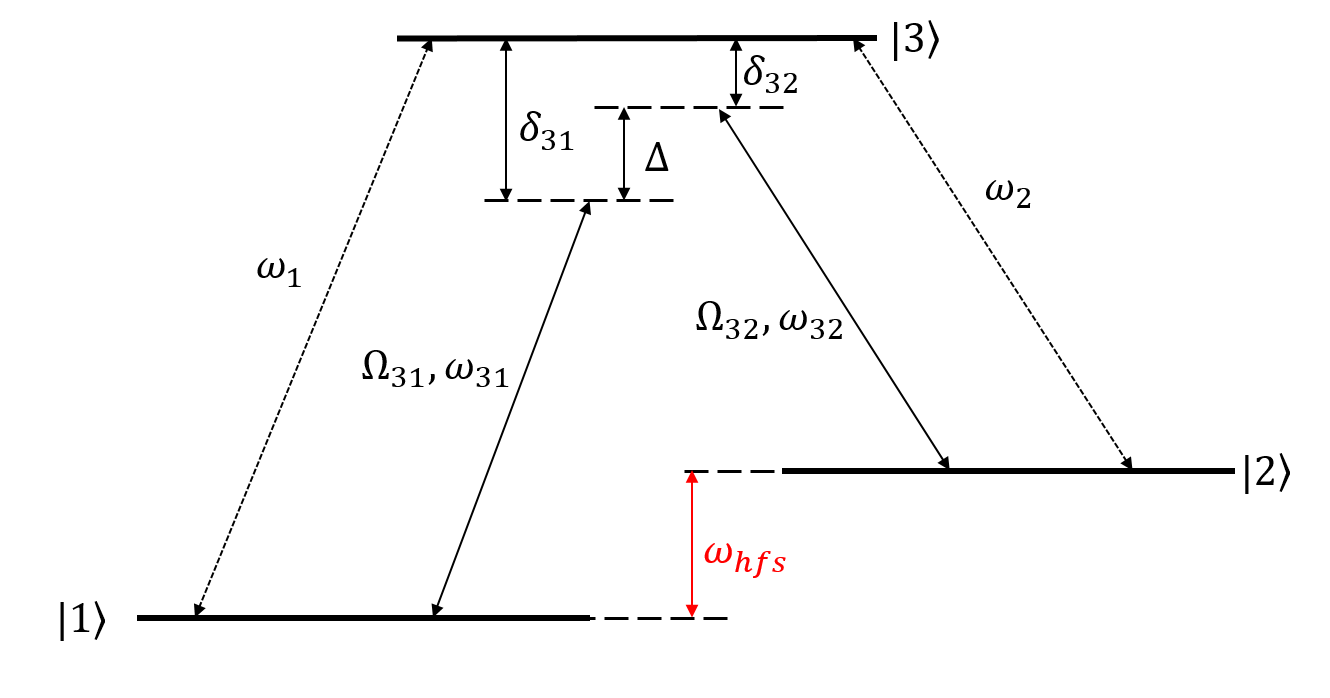
\includegraphics[height=0.23\textwidth,keepaspectratio]{lambdatransition}
\caption{\label{fig:lambdatransition}The three-level $\Lambda$ configuration of separate electric fields driving the $\ket{1}-\ket{3}$ and $\ket{2}-\ket{3}$ transitions.}
\end{figure}

Commercially available CSACs currently exploit CPT phenomenon $^[$\citep{articleb}$^]$. The $\Lambda$ configuration as shown in Fig. (\ref{fig:lambdatransition}) approximates the alkali atoms as a three-level system with separate electric fields driving $\ket{1}-\ket{3}$ and $\ket{2}-\ket{3}$ transitions. Parity of the ground states forbids $\ket{1}-\ket{2}$ transitions $^[$\citep{Khan2017CoherentEIT}$^]$. CPT occurs in a $\Lambda$ system when the relative detuning $\Delta=\delta_{31}-\delta_{32}=0$ of the electric fields enables pumping into a non-coupled coherent state $\ket{NC}$ $^[$\citep{Phillips:05}$^]$. 

The atom-light interaction for a two-level system where the interaction Hamiltonian in the dipole approximation is $\hat{H}_{I}=-\hat{\vec{d}}\cdot\hat{\vec{E}}$ where $\hat{\vec{d}}$ is the electric dipole moment and the electric field operator is $\hat{\vec{E}}=\hat{\vec{\epsilon}}E_{0}cos(\omega t)$. The Rabi frequency is derived as $\Omega=\frac{E_{0}}{\hbar}\bra{e}\hat{\vec{d}}\cdot\hat{\vec{\epsilon}}\ket{g}$. By extending the derivation to a $\Lambda$ system the approximate non-coupled dark state can be calculated. The Hamiltonian $H=H_{0}+H_{I1}+H_{I2}$ is derived as 
\begin{equation}
\label{eq:interactionham0}
\hat{H}_{0}=\sum_{i}\hbar\omega_{i}\ket{i}\bra{i},
\end{equation}
\begin{equation}
\label{eq:interactionham1}
\hat{H}_{I1}=\frac{\hbar\Omega_{31}}{2}(e^{i\omega_{31}t}\ket{3}\bra{1}+e^{-i\omega_{31}t}\ket{1}\bra{3}),
\end{equation}
\begin{equation}
\label{eq:interactionham2}
\hat{H}_{I2}=\frac{\hbar\Omega_{32}}{2}(e^{i\omega_{32}t}\ket{3}\bra{2}+e^{-i\omega_{32}t}\ket{2}\bra{3}),
\end{equation}


where $\hat{H}_{0}$ is the internal energy of the atoms $^[$\citep{Purves2006AbsorptionInterferometery}$^]$ . The eigenstates of $\hat{H}$ when $\omega_{31}-\omega_{32}=\omega_{hfs}$ are derived as $^[$\citep{Purves2006AbsorptionInterferometery}$^]$: THIS

\begin{equation}
\label{eq:CPTstatesC1}
\ket{C_{1}}=\frac{1}{\sqrt[]{2}}(\frac{\Omega_{31}}{\sqrt[]{\Omega_{31}^{2}+\Omega_{32}^{2}}}\ket{1}+\frac{\Omega_{32}}{\sqrt[]{\Omega_{31}^{2}+\Omega_{32}^{2}}}\ket{2}-\ket{3}),
\end{equation}
\begin{equation}
\label{eq:CPTstatesC2}
\ket{C_{1}}=\frac{1}{\sqrt[]{2}}(\frac{\Omega_{31}}{\sqrt[]{\Omega_{31}^{2}+\Omega_{32}^{2}}}\ket{1}+\frac{\Omega_{32}}{\sqrt[]{\Omega_{31}^{2}+\Omega_{32}^{2}}}\ket{2}+\ket{3}),
\end{equation}
\begin{equation}
\label{eq:CPTstatesNC}
\ket{NC}=\frac{\Omega_{32}\ket{1}-\Omega_{31}\ket}{\sqrt[]{\Omega_{31}^{2}+\Omega_{32}^{2}}}.
\end{equation}

Since $\ket{NC}$ is a superposition of the ground states, atoms pumped into this dark state become trapped. Population builds up in the dark state and eventually the atoms do not interact with the electric fields. The  transmission peak is observed at $\omega_{hfs}$. This simplified derivation does not fully describe the system, it is important to note that phase coherence between the electric fields is a requirement for CPT $^[$\citep{Khan2017CoherentEIT}$^]$. The evolution of the three-level system is derived using the Lindblad Master equation in Ref. [\citen{5423}] and Ref. [\citen{Fleischhauer2005ElectromagneticallyMedia}]. In ref. [\citen{Borges2017InfluenceTrapping}] the first order optical susceptibility $\chi^{(1)}$ is calculated, where $\chi^{(1)}$ applies for CPT and the typical regime of electromagnetically induced transparency (EIT) ($\Omega_{31}\gg \Omega_{32}$). The system absorption and dispersion is given by \textit{Im}$(\chi^{(1)})$ and \textit{Re}$(\chi^{(1)})$, respectively. 


Fig. (\ref{fig:CPTplot}) shows the absorption and dispersion plotted as a function of the relative detuning $\Delta=\omega_{31}-\omega_{32}-\omega_{hfs}$ where the sharp transmission peak at zero detuning enables locking of the LO to ground state resonance. This is experimentally achieved using a current-modulated diode laser which has an optical carrier frequency and a modulated frequency of $\omega_{hfs}/2$ to produce the first order sidebands separated by $\omega_{hfs}$. The laser frequency is tuned such that the first-order sidebands are resonant with the $\ket{1}-\ket{3}$ and $\ket{2}-\ket{3}$ transition $^[$\citep{Lutwak2002TheInterrogation}$^]$. 

\begin{figure}[t]
\centering
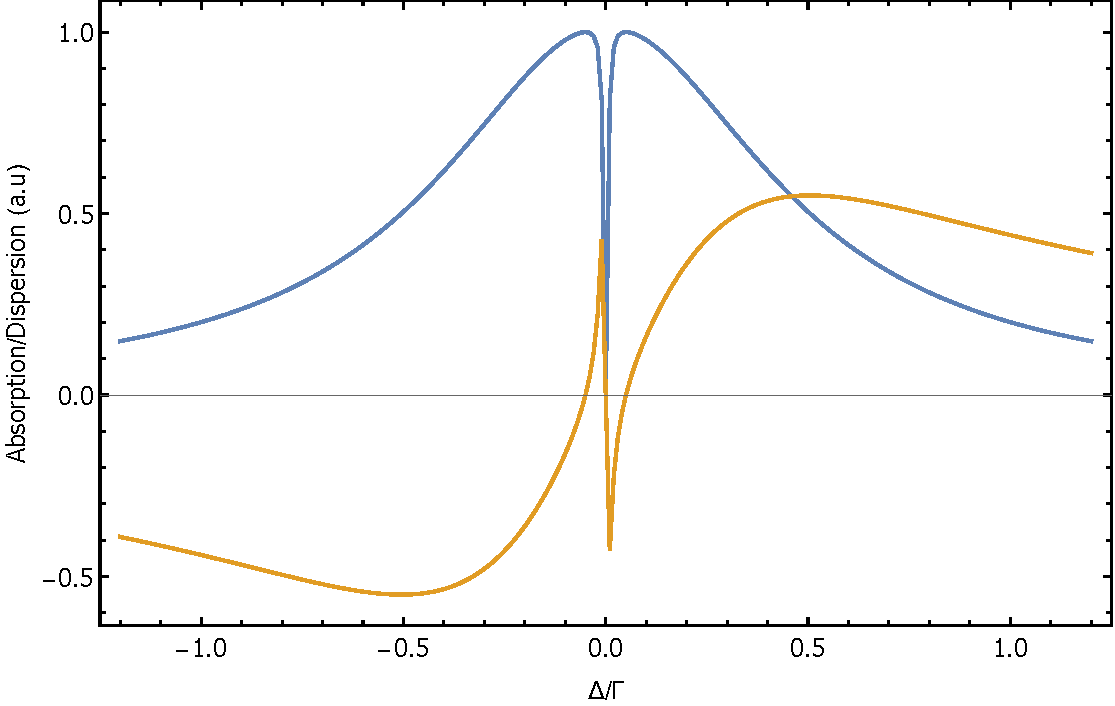
\includegraphics[height=0.27\textwidth,keepaspectratio]{CPTplot}
\caption{\label{fig:CPTplot}Theoretical absorption (blue) and dispersion (yellow/brown) as a function of $\Delta/\Gamma$ in the CPT regime ($\Omega_{31}\approx\Omega_{32}$) where $0.5\Gamma=\Gamma_{31}=\Gamma_{32}$.}
\end{figure}


\subsection{Frequency Stability}
Accuracy and stability are characteristics of an oscillator. Accuracy describes the offset from the ideal value, whilst stability defines the ability to produce the same value over a certain period of time $^[$\citep{Lombardi2001AnCalibrations}$^]$. The performance of CSACs relies upon the frequency stability over a certain integration time, the power consumption and the size of the device. The Allan deviation $\sigma_{y}$ provide a measure of the fractional frequency stability. In Ref. [\citen{Knappe2007MEMSClocks}] white frequency noise approximately describes the frequency stability when the averaging time $\tau$<100 s, such that:

\begin{equation}
\label{eq:AllanDev}
\sigma_{y}(\tau)=\frac{X}{Q(S/N)}\sqrt[]{\tau}.
\end{equation}

It is clear from Eq. (\ref{eq:AllanDev}) that frequency stability is dependent on the Lorentzian CPT transmission linewidth $\gamma$ and the amplitude.   
The quality factor $Q=\omega_{c} /\gamma$, the signal to noise ratio is $S/N$ and $X$ is the method of interrogation parameter. In addition, frequency stability depends on, for the case of $\tau\approx100 s$ and $\tau>100$ s the flicker noise floor ($\sigma_{y}\propto const$) and the frequency drift ($\sigma_{y}\propto\tau$), respectively.  

\begin{figure}[t]
\centering
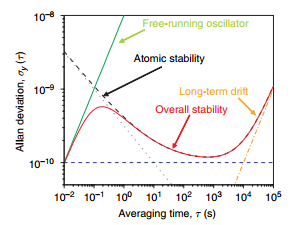
\includegraphics[height=0.37\textwidth,keepaspectratio]{frequencystability}
\caption{\label{fig:frequencystability} $\sigma_{y}$ of the locked oscillator (red) and for unlocked free-running oscillator (green). The atomic stability (black dashes) is modelled by the white noise (grey dots), flicker noise floor (blue dashes) and frequency drift (orange dot dashes) \citep{Knappe2007MEMSClocks}.}
\end{figure}




\section{\label{sec:level1}CSAC Research and Development}
%In addition, DR absorption $\gamma$ is larger than the CPT transmission %peak due Doppler and pressure broadening such that the overall absorption %for CPT and DR is an approximately Gaussian function yet the CPT %transmission feature is approximately Lorentzian.. 

%The DARPA CSAC outcomes from the main contributors and the other impactful research contributing to meeting the ultimate goal of producing a robust miniaturised atomic clock is examined 

%. Additionally, the current CSAC research and the future outlook following the launch of DAPRA's ACES is discussed in this section. 

\begin{figure}[b]
\centering
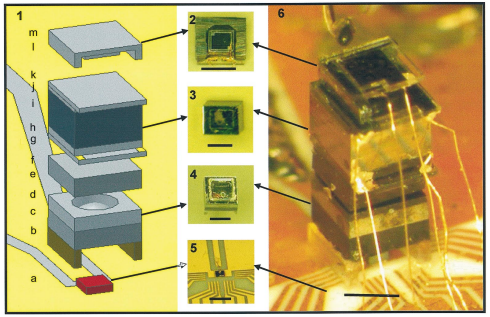
\includegraphics[height=0.27\textwidth,keepaspectratio]{NISTwafer}
\caption{\label{fig:NISTwafer}NIST CSAC physics package. (1) Schematic components: (a) VCSEL, (b) glass, (c)(d)(e)(f) $\lambda$/4 wave-plate optics, (g) indium-tin oxide (ITO) film, (h) glass, (i) Silicon, (j) glass, (k) ITO film, (l) glass, (m) glass. (2) photodiode, (3) $Cs$ vapor cell, (4) optics, (5) laser and (6) physics assembly where the scaling is shown by the 1mm black line $^[$\citep{Knappe2004AClock}$^]$.}
\end{figure}


Prior to beginning construction of the CSAC model, Symmetricom completed an experimental study of the potential for CPT or the conventional double-resonance (DR) technique, used previously in the Symmetricom X72 oscillator,  to meet the DARPA criteria $^[$\citep{Lutwak2002TheInterrogation}$^]$. The testing MEMS package contained a < 1 mm$^3$ vapour cell. $Cs$ were used due to the increased vapour pressure at the operating temperature $>$ 65 $^{\circ }\textrm{C}$ compared to $Rb$. Despite the CPT method having a resonance $\gamma$ approximately 1/2 that of the conventional method, DR was deemed the better technique to obtain short-term stability. This is due to the 10 times larger DR $S/N$ due to contributions of the carrier and second-order sidebands to the background level for CPT. However, Symmetricom express concern over the microwave cavity of the DR technique being the limiting factor to further reduce size. Symmetricom further investigates using CPT spectroscopy in Ref. [\citen{LutwakRandEmmonsDEnglishTRiley2003TheProgress}] determining that D1 line resonance increases the frequency stability compared to applying the laser field on the D2 line. 

\begin{figure}[b]
\centering
\begin{subfigure}[b]{0.45\textwidth}
   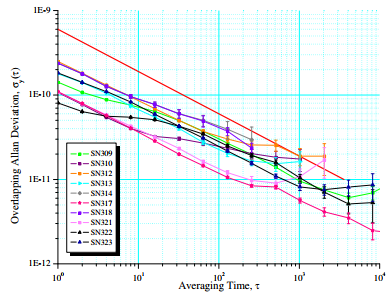
\includegraphics[width=1\linewidth]{shorttermstab}
	\caption{\label{fig:shorttermstab}}
\end{subfigure}
\begin{subfigure}[b]{0.45\textwidth}
   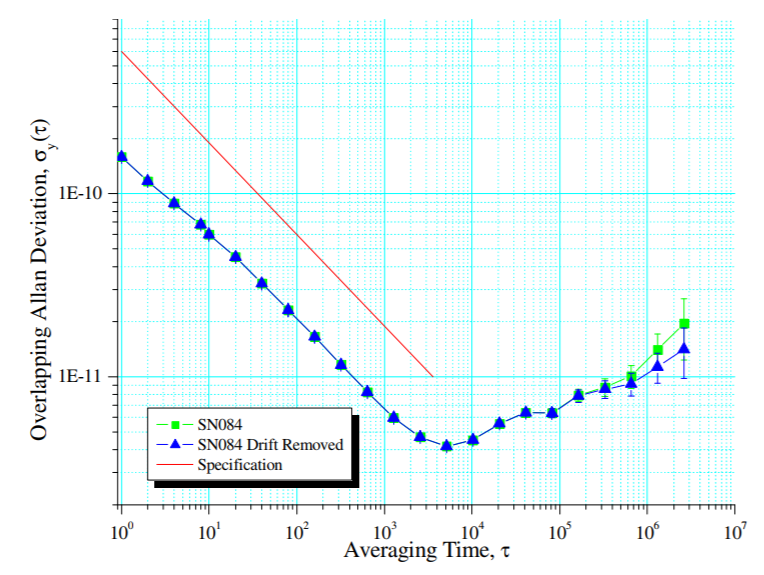
\includegraphics[width=1\linewidth]{longtermstab}
	\caption{\label{fig:longtermstab}}
\end{subfigure}
\caption[]{$\sigma_{y}(\tau$) for (a) short-term and (b) long-term (6 months) measurements where the drift linear component present (removed) in green (blue) $^[$\citep{LutwakR.RashedA.Varghese2007TheEvaluation}$^]$.}
\end{figure}



In 2004 the National Institute of Standards and Technology (NIST) revealed the first CSAC prototype with a 9.5 mm$^3$ volume MEMS fabricated physics package $^[$\citep{Knappe2004AClock}$^,$\citep{Gerginov2005Component-levelReference}$^]$. NIST pioneered the layered wafer structure fabrication of the physics package shown in Fig (\ref{fig:NISTwafer}) which requires 75 mW to operate, uses the CPT method and enables the production of many units at once. Implementation of 1 mm$^3$ $Cs$ vapor cell fabrication proposed by NIST in Ref. [\citen{Kitching2002MiniatureReference}] using anodic bonding of borosilicate glass and silicon (Si), instead of glass blowing techniques, reduces the cell size.  



In Ref. [\citen{Gerginov2005Component-levelReference}] improvements to the NIST physics package included the addition of the thermally isolating baseplate and a lithographic etching in tungsten film on the baseplate provided a heater below the VCSEL. This reduces the power required to operate the VCSEL. The CSAC prototype use a voltage-controlled oscillator (VCO) as the LO and control electronics implemented servo locking of the LO frequency only. The combined volume of physics package, the B-field coils and shielding was 0.7 cm$^{3}$. The CSAC prototype achieves short-term stability ($\tau$<100 s) of $6\times10^{-10}/\sqrt{\tau}$, total power consumption < 200 mW and has a 10 cm$^{3}$ volume.

Thereafter, Symmetricom produced their first prototype in 2005 with short term stability $\approx4\times 10^{-10}/\sqrt{\tau}$, power consumption <200 mW and 10 cm$^{3}$ volume $^[$\citep{LutwakTheClock}$^]$. The physics package was contained in a vacuum sealed ceramic lid to thermally isolate the components for military operation in ambient temperature ranging between -40 $^{\circ }\textrm{C}$ and 85 $^{\circ }\textrm{C}$ $^[$\citep{LutwakTheClock}$^]$. To make the CSAC more robust the the vapor cell is secured by polyimide tethers. To reduce the control electronics components required and thus the power consumption, a microprocessor is implemented with firmware code. Firmware algorithms demodulate and analyse the error signal of the CPT transmission peak to tune the LO.   



In 2007 in Ref. [\citen{LutwakR.RashedA.Varghese2007TheEvaluation}] the physics package assembly is updated from using "folded-optics" to a component assembly which is similar to the design in Fig. (\ref{fig:NISTwafer}). The $Cs$ transmission peak becomes more symmetric by removing reflection of the laser beam in the prior design. A performance study is undertaken of 10 CSACs, each with 125 mW operating power and 15 cm$^{3}$ volume. Shock testing of the CSAC inspects the cell suspension where all tested devices can sustain a shock up to 500g along all axes. The short-term stability of CSACs is shown in Fig. (\ref{fig:shorttermstab}) where the average stability is $\sigma_{y}(\tau$=1 s) < 1.6 $\times 10^{-10}$. In Fig. (\ref{fig:longtermstab}) $\sigma_{y}(\tau$) is measured for 6 months after the devices has already been operating for 6 months and to inspect the 10$^{12}$/day drift effect. Firmware has been updated proving further power and frequency control of the VCSEL using servo algorithms, complete autonomous locking and acquisition of control parameters.   


Development of other industrial CSAC prototypes includes: Honeywell (1.7 cm$^{3}$, 57 mW, $\sigma_{y}(\tau$=1 hour)=5$\times 10^{-12}$) $^[$\citep{Youngner2007AClock}$^]$ and Teledyne Scientific (< 1 mm$^{3}$, < 30 mW, $\sigma_{y}(\tau$=1 hour) < 10$^{-11}$ $^[$\citep{DeNatale2008CompactClock}$^]$. Ref. (\citen{Douahi2007VapourStandard}) explores 1mm$^{3}$ fabrication producing two cavities. One contains the metallic $Cs$ droplet and dispenses $Cs$ atoms to the other irradiates the cavity. The advantage of this process over the typical anodic bonding process is improved control of the cell atmosphere and $Cs$ purity. 

\begin{figure}[b]
\centering
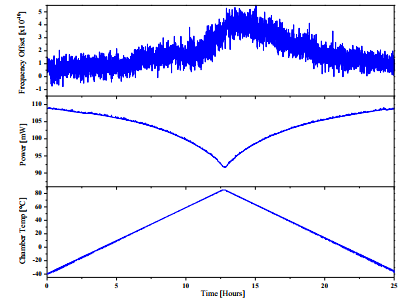
\includegraphics[height=0.32\textwidth,keepaspectratio]{tempplot}
\caption{\label{fig:tempplot}SA.45s performance for chamber temperature ranging between -40 $^{\circ }\textrm{C}$ to 85 $^{\circ }\textrm{C}$.}
\end{figure}

Symmetricom released the SA.45s CSAC commercial product in 2011 with $\sigma_{y}(\tau) < 2\times 10^{-10}/\sqrt{\tau}$, power consumption < 125 mW and volume < 17 cm$^{3}$ $^[$\citep{articleb}$^]$. The CSAC contains: the physics package, 10 MHz TCXO LO, a microprocessor package, a microwave synthesiser mounted on a printed circuit board (PCB). The microwave synethesiser contains the 4.6 GHz VCO which enables modulation of the VCSEL where the VCO is phase-locked to the LO. In addition to the 10 MHz LO output, a 1 pulse-per-second (PPS) output is added for applications requiring GNSS satellite synchronisation. An example of the performance measurements taken in a controlled-temperature environment is shown in Fig. (\ref{fig:tempplot}). The expectation is that low temperatures require more power to temperature control the laser and the vapour cell each with stabilised temperature of 85 $^{\circ }\textrm{C}$ \citep{LutwakR.RashedA.Varghese2007TheEvaluation}. However, the temperature isolation of physics package and efficiency of the electronics reduces the power.

In 2012 Gorecki employed the double cell micro-fabrication technique discussed in Ref. [\citep{Douahi2007VapourStandard}] to produce a CSAC with $\sigma_{y}(\tau$=1 hour) = 5$\times$ 10$^{-11}$, 200 mW power consumption and tens of cm$^{3}$ volume. 





\section{\label{sec:level1}Applications}
The development of CSACs has been driven by military applications including navigation when the GNSS signal has purposefully been jammed. This causes the civilian signal, which produces GNSS time ticking, to be rendered useless in this area. The development of GNSS receivers which contain a precise timing capable of maintaining, for a day, an accuracy within 1 ms of UTC enable direct military encrypted signal acquisition for precise positioning $^[$\citep{Fruehauf2001FastClock.}$^]$. CSAC technology therefore can also be used on unmanned aerial vehicles to provide hold-over in GNSS signal outages and prevention against military drone hijacking. Spoofing, which is controlling a target by sending a doctored GNSS signal to the GNSS receiver, has been demonstrated on a drone in Ref. [\citen{unknown}]. 

Jamming is achieved by applying a high power signal at the frequency of the receiver $^[$\citep{article}$^]$. Jamming of civilian GNSS signals is cause for concern in the financial sector, navigation of ships and airplane navigation. Ref. [\citen{Coffed2014TheUtility}] warns of the potential vulnerabilities of GNSS reliance, outlining cases where the illegal jamming devices have overridden GNSS signals used in airport tracking systems and disturbed trading-time stamping.

A selection of recent experimental investigations of the SA.45s CSACs is presented which aim to investigate implementation to satisfy scientific or industrial applications. Measurements of $\sigma_{y}(\tau$) of a selection of miniature atomic clocks, including SA.45s, was completed to calculate the power spectral density (PSD) coefficients of the individual clocks. In Ref. [\citen{Krawinkel2014ApplicationPositioning}] improved kinematic GNSS single point positioning (SPP) is achieved by modeling noise signals using the PSD coefficients applied to an Extended Kalman Filter (EKF). The CPT-GNSS receiver vertical-coordinate precision improves by 26.2 $\%$ when the receiver error is modelled using this technique.  
 
When the CSAC is used as the internal oscillator of the GNSS instead of TXCO, improvements to the synchronisation between the GNSS satellite and the receiver are expected. The GNSS satellite PPS is used for long-term discipline of the CSAC and reduces the drift of the CSAC. Ref. [\citen{Calero2016PositioningSystems}] the CSAC was determined to provide an approximate positioning using only three satellites, instead of requiring four satellites, during static and dynamics testing. 

Temperature calibration of CSAC is completed in Ref. [\citen{Fernandez2017CSACPerformance.}] such that an environmental steering value can be implemented in addition to the frequency drift steering using PPS discipling. Steering for changes in the environment greatly improves stability of the CSAC compared to without. During outages of the GNSS signal > 1 minute the CSAC enables a considerably faster recovery of GNSS receiver positioning compared to the TXCO case. However, concern is expressed for correcting for aging of the CSAC devices. 

An area of application where CSACs are expected to improve timing is in underwater sensing $^[$\citep{Gardner2012AdvancementsOscillators}$^]$. 6 months underwater timing of 13 ocean–bottom seismographs (OBS) each containing a CSAC were compared using the Seascan microprocessor compensated crystal oscillator. The CSAC provided promises high timing accuracy results. However, the study is extended to include 38 CSACs and continued measurements from the original stage up to 4.5 years. Only 5 of the second deployment clocks meet the aging specification required therefore the reliability of the devices is questioned. Concern is expressed in each report for the temperature stability as the vacuum degradation, correcting for changing drift rate and the retraceability. retraceability is the variation in the drift response after switching the device off and back on again $^[$\citep{Gardner2016ATiming}$^]$.   










































\section{\label{sec:level1}Outlook}
The ACES program aims to improve the limiting factors of the CSACs operation. These limitations for SA.45s include: the requirement for lengthy calibration each time the device is switched on due to the poor retraceability and inability to predict or correct long-term frequency drifting. In addition, the program intends to investigate pioneering methods of interrogation and atomic confinement $^[$\citep{DARPA2016Broad}$^]$. OEwaves has received funding from the ACES to continue exploring approaches of using a  whispering gallery mode (WGM) micro-resonator to produce a miniature $Rb$ atomic clock $^[$\citep{Maleki2010All-opticalClock}$^,$\citep{Maleki2011All-OpticalClock}$^]$.

The majority of SA.45s CSAC were unable to satisfy the requirements for long-term oceanic deployment due to failure or partial loss of the vacuum. In addition, frequency drifting due component aging is an additional problem when precision timing for the duration of typically 2 year deployments is required. Further improvements to the fabrication of the physics package may enable these devices to withstand underwater conditions. Further testing of the underwater aging of CSACs is necessary to gain a better expectation of frequency drifting so that changes could be made to the device components or correction algorithms could be implemented. The results of replacing TCXO in GNSS receivers with CSAC show considerable benefits particularly in limited GNSS signals. This is due to the short-term CSAC stability, $\sigma_{y}(\tau) < 2\times 10^{-10}/\sqrt{\tau}$ and long-term steering of CSAC using precision timing of GNSS satellite atomic clocks.

\begin{acknowledgements}
I would like to thank Dr Luca Marmugi and Dr Paul Griffin for helpful discussions. I would also like thank Prof Patrick Gill and his colleagues at NPL for giving me a tour of the atomic clocks laboratories and for useful discussions.   
\end{acknowledgements}


\bibliographystyle{ieeetr}

\bibliography{main}

\end{document}